%Dies ist die Hauptseite des Dokumentes. Es werden u. a. alle Kapitel, Einstellung im Header eingebunden.
%Ver�nderungen m�ssen in folgenden Dateien vorgenommen werden:
			%- Layout.tex 
			%- newComments.tex
			%- Titelseite
			%- Versions�bersicht
			%- einzelne Kapitel (evtl. erweitern) 
			
			
% Definition von globalen Parametern, die derzeit auf der Titelseite und in der Kopfzeile 
% verwendet werden. Der in <> gesetzte Text ist zu ver�ndern.  

\newcommand{\praktikumTitel}{<Titel des Praktikums>}
\newcommand{\projektTitel}{<Titel des Teilprojektes>}


%Hier sind alle Einstellungen enthalten, die sich auf das Seiten- und Dokumentenlayout beziehen

\documentclass[
	11pt,								% Schriftgr��e
	DIV12,
	german,							% f�r Umlaute, Silbentrennung etc.
	oneside,						% einseitiges Dokument
	titlepage,					% es wird eine Titelseite verwendet
	halfparskip,				% Abstand zwischen Abs�tzen (halbe Zeile)
	normalheadings,			% Gr��e der �berschriften verkleinern
	tablecaptionabove,	% Beschriftung von Tabellen unterhalb ausgeben
	final								% Status des Dokuments (final/draft)
]{scrreprt}						% 


%------�ndern von Schriftschnitten - (Muss ganz am Anfang stehen !) -------------
\usepackage{fix-cm}

%------Umlaute ------------------------------------------------------------------
% 	Umlaute/Sonderzeichen wie ���� k�nnen direkt im Quelltext verwenden werden.
%		Erlaubt automatische Trennung von Worten mit Umlauten.
\usepackage[T1]{fontenc}								 
\usepackage[latin1]{inputenc}

%------Anpassung der Landessprache-----------------------------------------------
\usepackage{ngerman}

%------Einfache Definition der Zeilenabst�nde und Seitenr�nder-------------------
\usepackage{geometry}
\usepackage{setspace}
\usepackage{tocbasic}

%------Schriftgr��enanpassung von einzelnen Textpassagen-------------------------
\usepackage{relsize}

%------Trennlinien in Kopf- und Fusszeile
\usepackage[headsepline, footsepline, ilines]{scrpage2}

%------Grafiken------------------------------------------------------------------
\usepackage{graphicx}
\usepackage{float}

%------Packet zum Sperren, Unterstreichen und Hervorheben von Texten------------
\usepackage{soul}

%------erg�nzende Schriftart----------------------------------------------------
\usepackage{helvet}

%------Lange Tabellen-----------------------------------------------------------
\usepackage{longtable}
\usepackage{array}
\usepackage{ragged2e}
\usepackage{lscape}

\usepackage{xparse}
\usepackage{framed}
\usepackage[usenames,dvipsnames]{color}

%------PDF-Optionen-------------------------------------------------------------
\usepackage[
	bookmarks,
	bookmarksopen=true,
	colorlinks=true,
	linkcolor=black,				% einfache interne Verkn�pfungen
	anchorcolor=black,			% Ankertext
	citecolor=black, 				% Verweise auf Literaturverzeichniseintr�ge im Text
	filecolor=black, 				% Verkn�pfungen, die lokale Dateien �ffnen
	menucolor=black, 				% Acrobat-Men�punkte
	urlcolor=black, 				% Farbe f�r URL-Links
	backref,								% Zur�cktext nach jedem Bibliografie-Eintrag als Liste von �berschriftsnummern
	pagebackref,						% Zur�cktext nach jedem Bibliografie-Eintrag als Liste von Seitenzahlen
	plainpages=false,				% zur korrekten Erstellung der Bookmarks
	pdfpagelabels,					% zur korrekten Erstellung der Bookmarks
	hypertexnames=false,		% zur korrekten Erstellung der Bookmarks
	% linktocpage 						% Seitenzahlen anstatt Text im Inhaltsverzeichnis verlinken
	]{hyperref}



			% enth�lt eingebundene Packete

%------Seitenr�nder-------------------------------------------------------------
\geometry{verbose, 										% zeigt die eingestellten Parameter beim Latexlauf an
			paper=a4paper, 									% Papierformat			
			top=25mm, 											% Rand oben
			left=25mm, 											% Rand links
			right=25mm, 										% Rand rechts
			bottom=45mm, 										% Rand unten
			pdftex													% schreibt das Papierformat in dei Ausgabe damit Ausgabeprogramm Papiergr��e erkennt		
	} 
	
%Seitenlayout
\onehalfspace        % 1,5-facher Abstand  

%------Kopf- und Fu�zeilen ------------------------------------------------------
\pagestyle{scrheadings}

%------Kopf- und Fu�zeile auch auf Kapitelanfangsseiten -------------------------
\renewcommand*{\chapterpagestyle}{scrheadings}

%------Schriftform der Kopfzeile ------------------------------------------------
\renewcommand{\headfont}{\normalfont}

%------Kopfzeile-----------------------------------------------------------------
\setlength{\headheight}{21mm}				% H�he der Kopfzeile
\ihead{\large{\textsc{\praktikumTitel}}\\		% Text in der linken Box
			 \small{\projektTitel}}
\chead{}														% Text in der mittleren Box

%----Fusszeile
\cfoot{}														% Text in mittlerer Box
\ofoot{\pagemark}										% Seitenzahl in rechter Box			





					% Diese Datei enth�lt alle Layouteinstellungen

%------Beginn des Gesamtdokumentes--------------------------------------------------------
\begin{document}

%------Eingebundene Seiten, Verzeichnisse bzw. Kapitel------------------------------------
%----Stil dieser Seite--------------------------------------------------------------------
\thispagestyle{plain}			% Kopfzeile bleibt leer

%----Beginn der Titelseite----------------------------------------------------------------
\begin{titlepage}

%----zentrierte Ausrichtung �ber die gesamte Seite----------------------------------------		
\begin{center}

%----Titel des Praktikum (\praktikumTitel in newComments zu ver�ndern)--------------------
{\relsize{4}{\textbf{\textsc{\praktikumTitel}}}}\\[5ex]

%----Titel des Teilprojektes (\projektTitel in newComments ver�ndern)---------------------
{\relsize{3}{\textbf{\textsc{\projektTitel}}}}\\[5ex]

Praxis der Softwarentwicklung\\
Sommersemester 2014\\[6ex]

{\relsize{3}\so{\textbf{Qualit�tssicherung}}}\\[5ex]

%----Titelbild------------------------------------------------------------

\includegraphics[scale=0.25]{bilder/logo.png}\\[5ex]

%----Daten des Auftraggebers
Auftraggeber\\[2ex]															
KIT - Karlsruher Institut f�r Technologie\\
Fakult�t f�r Informatik\\										
Institut f�r Anthropromatik und Robotik (IAR)\\
Intelligente Prozessautomation und Robotik (IPR)\\[2ex]
Betreuer: Andreas Bihlmaier\\
andreas.bihlmaier@gmx.net\\[5ex]

% ----Tabelle Teilnehmer---------------------------------------------------
Auftragnehmer\\

\begin{tabular}{l<{\hspace{20mm}} l<{\hspace{30mm}}}\\	
	Name 									& 	E-Mail-Adresse\\			% Zeilen�berschift
		
	\hline										% Linie unterhalb der Zeilen�berschrift
	
	%----Nachfolgend alle Namen und E-Mail-Adressen der Teilnehmer einf�gen	
	Alex Weber & alex.weber3@gmx.net\\
	Matthias Hadlich & matthias.hadlich@student.kit.edu\\
	Matthias Klatte	& matthias.klatte@go4more.de\\
	Micha Wetzel & micha.wetzel@student.kit.edu\\	
	Sebastian Kneipp &	sebastian.kneipp@gmx.net
	
	
\end{tabular}\\[2ex]

\end{center}

\vfill Karlsruhe, 22.09.2014

\end{titlepage}
											% Titelseite	
%kp ob wir des brauchen

%----�berschrift------------------------------------------------------------
{\relsize{2}\textbf{Versions�bersicht}}\\[2ex] 	

%----Start der Tabelle------------------------------------------------------
\begin{longtable}{|m{1.78cm}|m{1.59cm}|m{2.86cm}|m{1.9cm}|m{5.25cm}|}

	\hline																							% Linie oberhalb	
	
	%----Spalten�berschriften------------------------------------------------
	\textbf{Version}	&		\textbf{Datum}	&		\textbf{Autor}	&		\textbf{Status}	&		\textbf{Kommentar}	\\	%Spalten�berschrift	
	\hline																							% Gitterlinie
	
	%----die nachfolgeden beiden Zeilen so oft wiederholen und die ... mit den entsprechenden Daten zu f�llen wie erforderlich
	...		&		...		&		...		&		...		&		...\\				% Eintrag in Zeile
	\hline																							% Gitterlinie unten
	
%----Ende der Tabelle------------------------------------------------------	
\end{longtable}

				% Versions�bersicht

\tableofcontents													% Inhaltsverzeichnis wird automatisch generiert
\listoffigures														% ebenso das Abbildungsverzeichnis					

%----Kapitel des Feinentwurfs, die mit Inhalt zu f�llen sind------------------------------
\chapter{Zielbestimmung}

Die zu entwickelnde Softwarel�sung soll sich als �berwachungsinstrument in die Robot Operating System (ROS) Middleware einf�gen. Dabei soll �berwacht werden, ob jeder Prozess, der im ROS-Netzwerk enthalten ist, definierten Sollwerten entsprechend ordnungsgem�� Daten �bermittelt.\\
Gerade durch die gegebene Problematik eines auf mehrere Hosts verteilten Systems, bereitet das Erfassen und Verstehen von auftretenden Problemen zum aktuellen Stand des ROS Schwierigkeiten. Das vorliegende Projekt erfasst den Ist-Zustand der Prozesse im ROS-Netzwerk ohne Leistungseinbu�en kontinuierlich und visualisiert diesen im Vergleich zu definierten Soll-Werten. Auftretende Fehler und Abweichungen der von den Spezifikationen werden den Benutzer deutlich angezeigt. Es lassen sich Gegenma�nahmen f�r verschiedene Fehler definieren.\\

\section{Musskriterien}
\begin{itemize}
	\item Minimale Erweiterung bestehender Knoten zur �bermittlung von Metadaten
	\item Publizierung der Metadaten mit defnierter Frequenz auf Topics
	\item Deaktivierung der Datenerfassung einzelner Knoten
	\item Definition von Soll-Zust�nden
	\item Graphische �bersicht �ber Abweichungen von Soll- und Ist-Zustand der Knotendaten
	\item Statuserfassung der Host-Computer
\end{itemize}

\section{Wunschkriterien}
\begin{itemize}
	\item �berwachung weiterer ROS Bestandteile: Service, Parameters
	\item Selbstkontrolle der Knoten
	\item Ist-Zustand als Soll-Zustand definieren
	\item Erg�nzende �bersichten mit dem ROS Graphen und Plots �ber den zeitlichen Verlauf
\end{itemize}

\section{Abgrenzungskriterien}
\begin{itemize}
	\item Das Projekt wird keine vollst�ndige Automatisierung in Fehlerf�llen umsetzen.
	\item �berwachung der Netzwerkinfrastruktur
	\item Die Metadatenerfassung umfasst nur Knoten die daf�r modifiziert werden.
\end{itemize}
						% Kapitel 1
\chapter{Produkteinsatz}

\section{Anwendungsbereiche}
Angewandt wird die Software zum Suchen von Fehlern und �berwachen kompletter ROS Netzwerke.

\section{Zielgruppen}
Die Zielgruppe besteht aus Entwicklern und Administratoren von Umgebungen, in denen ROS eingesetzt wird. Es wird technisches Verst�ndnis der Nutzer vorausgesetzt. 

\section{Betriebsbedingungen}
\begin{itemize}
\item Zur Fehlererkennung wird die Software gestartet, um eine genauere Ursache des Fehlers festzustellen.
\item W�hrend des Produktivbetriebs wird die �berwachung zugeschaltet, um Versagen in dem System zu erkennen und automatische Gegenma�nahmen einzuleiten.
\end{itemize}
						% Kapitel 2
% Kapitel 3
%------------------------------------------------------------------------------------
\chapter{Produkt�bersicht}				% Kapitel 3
\chapter{Produktfunktionen}
Produktfunktionen hier\\
\\
also was kann unser produkt kleine beschreibung
				% Kapitel 4
\chapter{Produktdaten}

hier bin ich mir nicht ganz so sicher was genau rein muss							% Kapitel 4
% Kapitel 6
%-----------------------------------------------------------------------------------------

\chapter{Produktleistungen}				% Kapitel 4
% Kapitel 7
%-------------------------------------------------------------------------------


\chapter{Qualit�tsanforderungen}	% Kapitel 4
\chapter{Benutzeroberfl�che}

hier kommen dann ein paar bilder und dazugeh�rige beschreibungenen unserer gui

\begin{itemize}
	\item blasdgfs
	\item sdfg
	\item was man halt alles so allgemeines reinschreiben kann
\end{itemize}

\newpage

\begin{figure}

\section{Skizzen bzw. Bilder}

\subsection{name des bildes}
	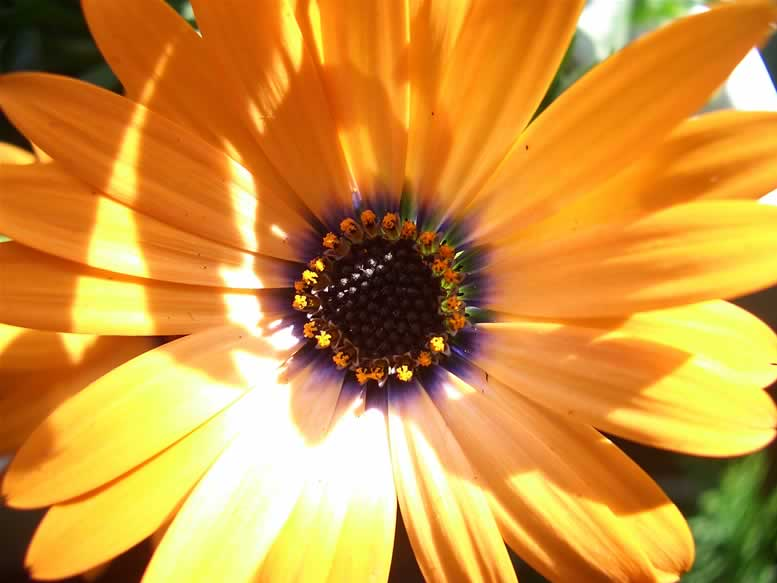
\includegraphics[width=\linewidth]{bilder/blume-beispielbild.jpg}
	\caption{bildunterschrift}
	
	Ein ganz ganz langer text zum bild\\
	kdfnakgflkadshfkjsfkljsadfjk�adshf�lkdf\\
	hsgkj�ldhflkghsfdlkgh�dklfhglkdsjgl�dshgkdsfh�gh\\
	sdflkendgkjhdsfk�ghadfsopfghaoifhaigtfuiaerhgiuag
\newpage

\end{figure}

\begin{figure}
\subsection{name des bildes}
	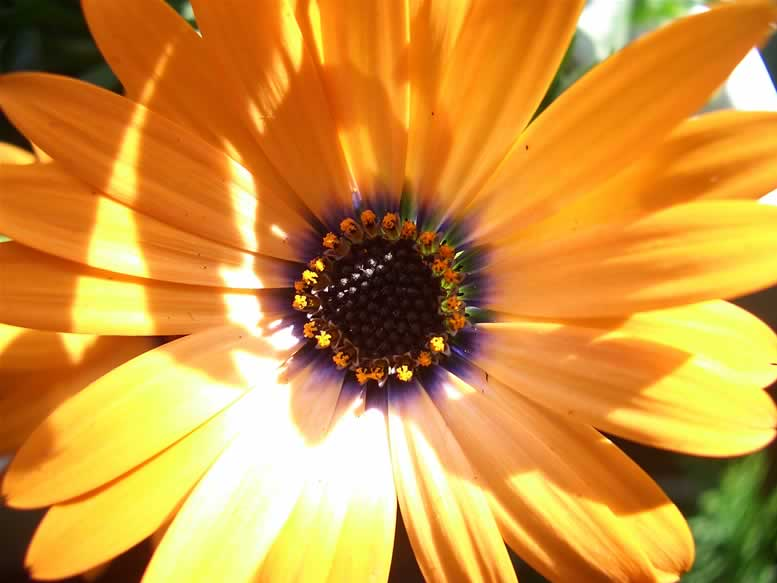
\includegraphics[width=\linewidth]{bilder/blume-beispielbild.jpg}
	\caption{bildunterschrift}
	
	Ein ganz ganz langer text zum bild\\
	kdfnakgflkadshfkjsfkljsadfjk�adshf�lkdf\\
	hsgkj�ldhflkghsfdlkgh�dklfhglkdsjgl�dshgkdsfh�gh\\
	sdflkgkjhdsfk�ghadfsopfghaoifhaigtfuiaerhgiuag
\newpage

\end{figure}
	
											% Kapitel 4
% Kapitel 9
%------------------------------------------------------------------------------------------

\chapter{Nichtfunktionale Anforderungen}						% Kapitel 4
\chapter{Produktumgebung}

\section{Software}
\subsection{Implementierung}
\begin{itemize}
  \item GNU/Linux (Ubuntu 12.04) oder neuer
  \item ROS Hydro oder neuer
  \item Python 2.7.3
  \item QT 4.8
  \item PyQT 4.9.1
\end{itemize}

\subsection{Dokumentation}
\begin{itemize}
  \item Latex
  \item Pydoc
\end{itemize}

\section{Lizenz}
Das Projekt wird BSD-Lizensiert. Sollte das durch den Einsatz bestimmter Bibliotheken nicht m�glich sein, wird die n�chstm�gliche freie Open-Source Lizenz, welche sich mit der Bibliothek vereinbaren l�sst, eingesetzt.
					% Kapitel 4

%------Ende des Dokumentes----------------------------------------------------------------
\end{document}
